\chapter{Captures des interfaces}
\label{chap:interfaces}

\section*{Introduction}

Ce chapitre présente le résultat visuel de \ProjectName{} et complète la
description technique du chapitre précédent. Les captures ne servent donc pas à
prouver une règle métier ou un échange protocolaire : elles montrent la manière
dont les fonctions réalisées sont organisées pour les utilisateurs. Les trois
captures strictement techniques du commissioning, de la connexion au simulateur
SAP et de la télémétrie OCPP restent volontairement dans le
chapitre~\ref{chap:implementation} afin d'éviter toute duplication.

\section{Page d'accueil}

La page d'accueil constitue le point d'entrée public de \ProjectName{}. Elle
présente directement le domaine de la plateforme à travers une photographie de
bornes de recharge, une proposition de valeur concise et un aperçu du pilotage
opérationnel. La navigation conduit aux capacités du produit, aux ressources et
au contact, tandis que les actions principales distinguent la connexion, la
création d'un compte client et la demande de démonstration destinée à une future
organisation.

\begin{figure}[H]
  \centering
  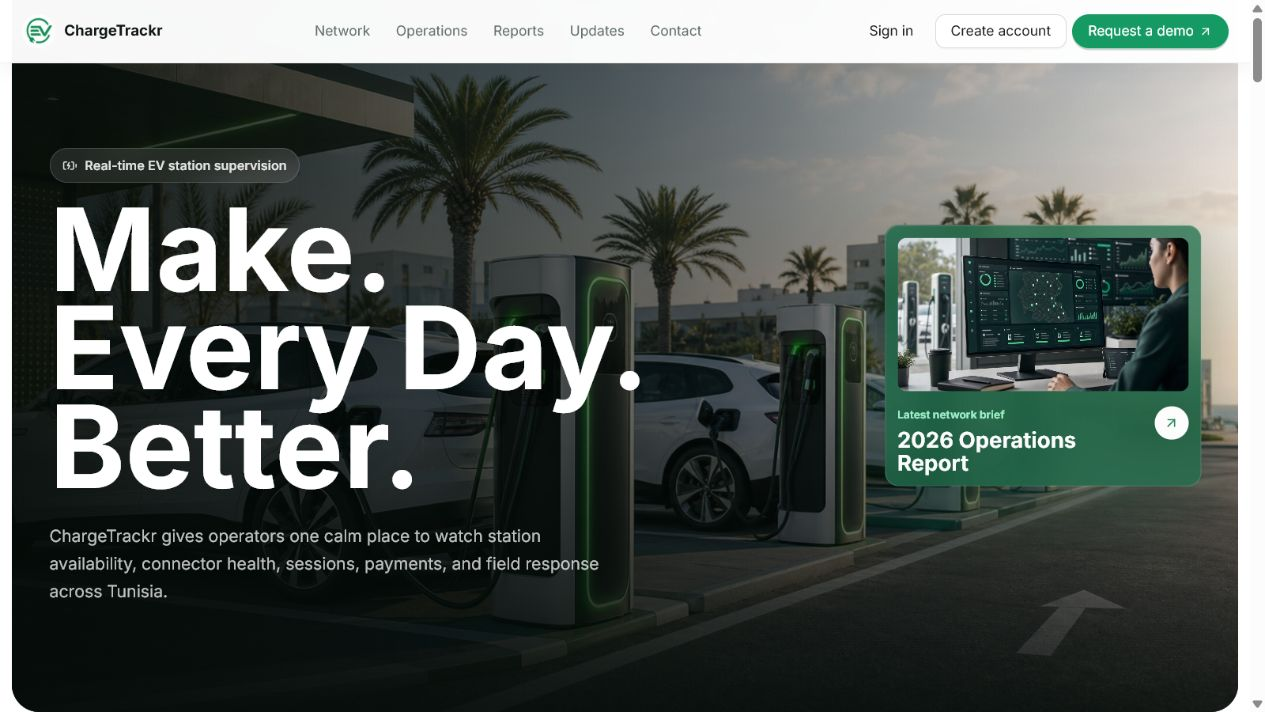
\includegraphics[width=0.98\textwidth]{assets/screenshots/landing-page.png}
  \caption{Page d'accueil publique de \ProjectName{}}
  \label{fig:interfaces-landing-page}
\end{figure}

Le premier écran privilégie la compréhension immédiate du service et conserve les
actions essentielles au-dessus de la ligne de flottaison. Les sections suivantes
détaillent la supervision temps réel, la gestion des opérations, les indicateurs
et le fonctionnement général. Cette entrée publique reste séparée de la coque
authentifiée afin de ne pas exposer la navigation métier avant la connexion.

\section{Entrée et prise en main}

Les pages publiques donnent accès à la présentation du produit, à la demande de
démonstration, à la connexion locale ou Google et à la création d'un compte
client. Après l'authentification, un onboarding court remplace la visite
exhaustive des fonctionnalités. Il rappelle le contexte d'accès, demande
uniquement les informations utiles au rôle et conduit vers une première action
concrète.

\begin{figure}[H]
  \centering
  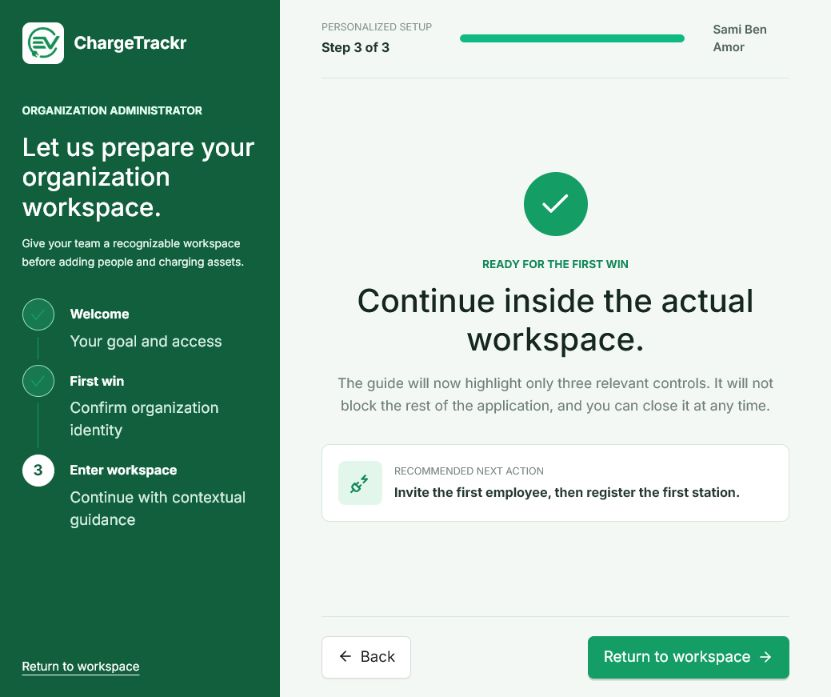
\includegraphics[width=0.92\textwidth]{assets/screenshots/onboarding-welcome.png}
  \caption{Onboarding personnalisé de l'administrateur}
  \label{fig:interfaces-onboarding}
\end{figure}

La progression reste visible dans la colonne latérale et les étapes déjà
terminées peuvent être identifiées immédiatement. L'utilisateur peut quitter le
parcours sans perdre l'accès à son espace. Pour un administrateur, la première
valeur consiste à confirmer l'organisation, inviter son équipe et préparer son
premier actif ; pour les autres rôles, les contenus sont adaptés à leur mission.

\section{Navigation et adaptation aux rôles}

La coque applicative reste commune afin de réduire l'effort d'apprentissage :
logo et menu principal à gauche, recherche et notifications en haut, contenu
contextuel au centre. Cette cohérence ne signifie pas que tous les utilisateurs
reçoivent le même tableau de bord. Les routes, indicateurs et actions sont
composés à partir du rôle et du périmètre autorisé.

\begin{table}[H]
  \centering
  \caption{Orientation des interfaces selon le rôle}
  \label{tab:interfaces-role-orientation}
  \begin{tabularx}{\textwidth}{@{}p{3.2cm}Y Y@{}}
    \toprule
    \textbf{Rôle} & \textbf{Priorité de l'interface} &
    \textbf{Actions mises en avant}\\
    \midrule
    Super administrateur & Gouvernance de la plateforme et portefeuille
    d'organisations & Traiter les demandes, gérer les organisations, contrôler
    les intégrations et les paramètres globaux.\\
    Administrateur & Pilotage métier d'une organisation & Gérer les employés,
    les actifs, les tarifs, l'abonnement commercial et les rapports.\\
    Opérateur & Continuité du service & Superviser les stations, qualifier les
    alertes, commander les bornes et affecter les interventions.\\
    Technicien & Exécution du travail terrain & Consulter les missions, mettre à
    jour leur avancement, joindre les preuves et soumettre un rapport.\\
    Client & Recharge et dépenses personnelles & Rechercher une station,
    démarrer une recharge, suivre la session, payer et consulter les reçus.\\
    \bottomrule
  \end{tabularx}
\end{table}

\section{Pilotage de l'organisation}

Le tableau de bord de l'administrateur associe un bandeau de période, l'identité
de l'organisation, des raccourcis opérationnels et des indicateurs vérifiés.
L'espace utilise la largeur disponible pour présenter les informations sans
empiler inutilement des cartes. Les résultats restent néanmoins séparés par
famille afin de faciliter la lecture.

\begin{figure}[H]
  \centering
  
\includegraphics[width=0.94\textwidth]{assets/screenshots/admin-overview.png}
  \caption{Tableau de bord de l'administrateur d'organisation}
  \label{fig:interfaces-admin-dashboard}
\end{figure}

La recherche globale, le centre de notifications et le profil restent accessibles
sans changer de contexte. Les raccourcis conduisent vers des workflows complets,
par exemple la création d'un employé, l'enregistrement d'une station ou la
génération d'un rapport.

\section{Stations et exploitation opérationnelle}

L'inventaire des stations permet de basculer entre carte, grille, liste et table.
Chaque mode répond à un besoin distinct : repérer géographiquement un actif,
comparer rapidement quelques stations ou exploiter un ensemble plus dense. Les
filtres et la recherche sont partagés entre les vues.

\begin{figure}[H]
  \centering
  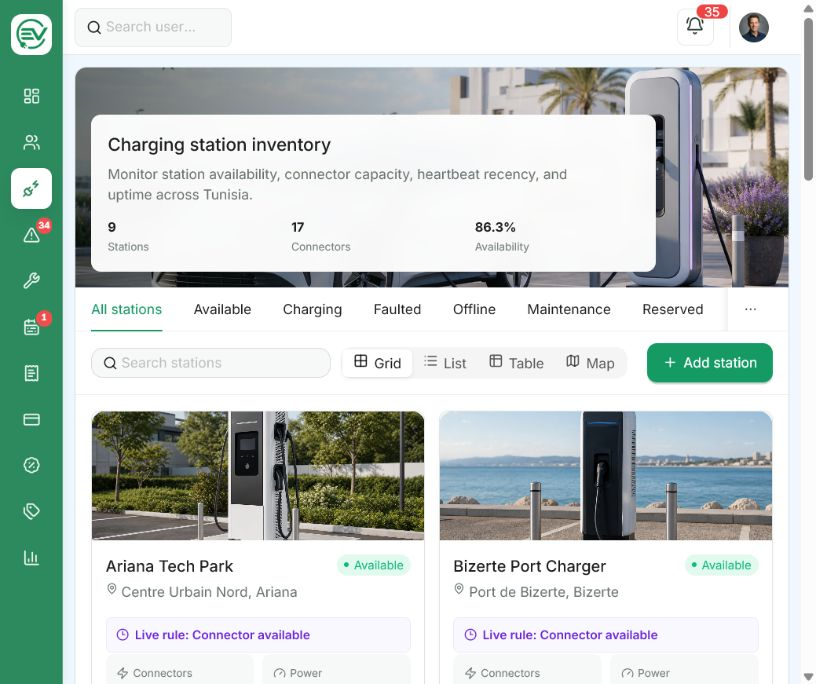
\includegraphics[width=0.94\textwidth]{assets/screenshots/stations-workspace.png}
  \caption{Inventaire des stations avec disponibilité calculée}
  \label{fig:interfaces-station-inventory}
\end{figure}

Les états visibles ne sont pas saisis dans l'interface. Ils proviennent des
projections décrites au chapitre précédent. Les actions de création et de
commissioning sont proposées à l'administrateur et à l'opérateur, alors que le
technicien dispose d'une consultation orientée diagnostic et que le client ne
voit que les stations utilisables.

Le centre d'alertes conserve la liste et le détail dans le même écran. Cette
disposition permet de qualifier plusieurs événements sans perdre les filtres, la
sélection ou la chronologie.

\begin{figure}[H]
  \centering
  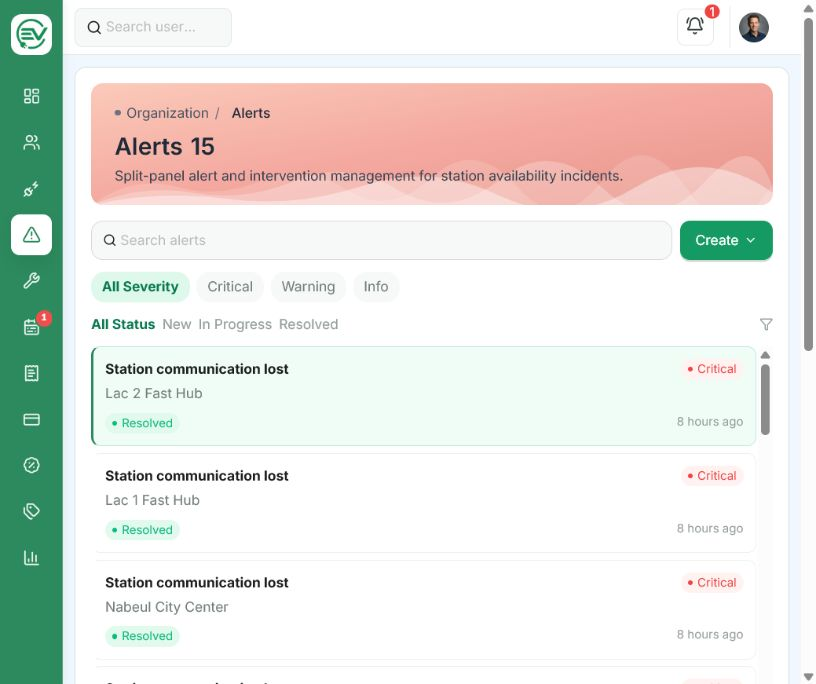
\includegraphics[width=0.94\textwidth]{assets/screenshots/alerts-workspace.png}
  \caption{Centre opérationnel des alertes}
  \label{fig:interfaces-alerts}
\end{figure}

La couleur indique la sévérité ou l'état, mais elle n'est jamais l'unique
information disponible : les libellés, références, dates et actions restent
explicites. Les compteurs de navigation attirent l'attention sans remplacer le
filtrage de la page.

\section{Gestion commerciale et reporting}

L'abonnement de l'organisation est séparé des paiements des conducteurs. La page
commerciale présente le plan courant, la période d'évaluation ou de facturation,
les capacités consommées et les demandes de changement. Cette séparation rend
le rôle financier de chaque écran explicite.

\begin{figure}[H]
  \centering
  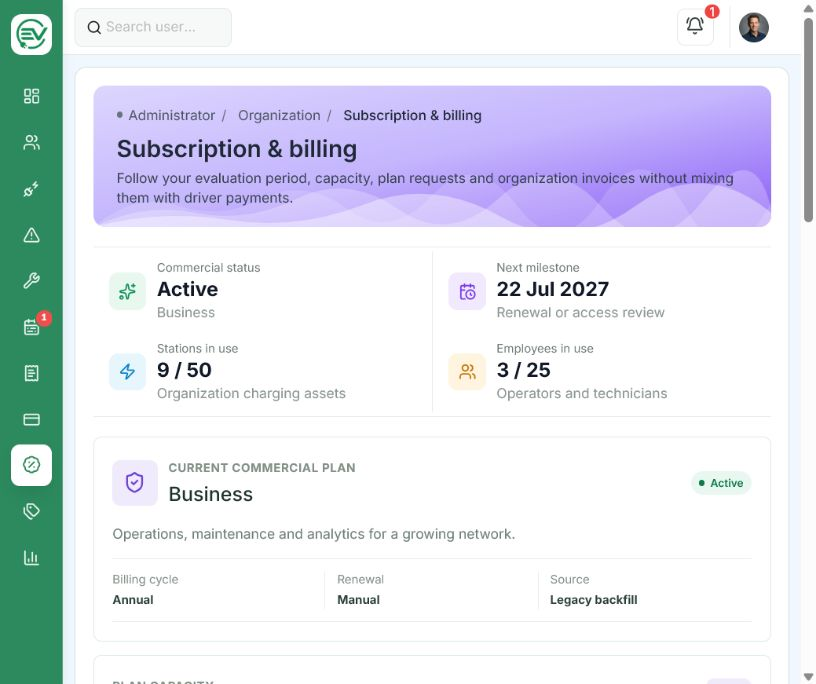
\includegraphics[width=0.94\textwidth]{assets/screenshots/organization-billing.png}
  \caption{Suivi de l'abonnement commercial de l'organisation}
  \label{fig:interfaces-organization-billing}
\end{figure}

Le studio de performance complète le tableau de bord sans le dupliquer. Il
propose des indicateurs plus détaillés, des répartitions, des tendances et des
filtres de période. Les rapports internes peuvent ensuite être composés,
accompagnés de pièces jointes et transmis dans le périmètre de l'organisation.

\begin{figure}[H]
  \centering
  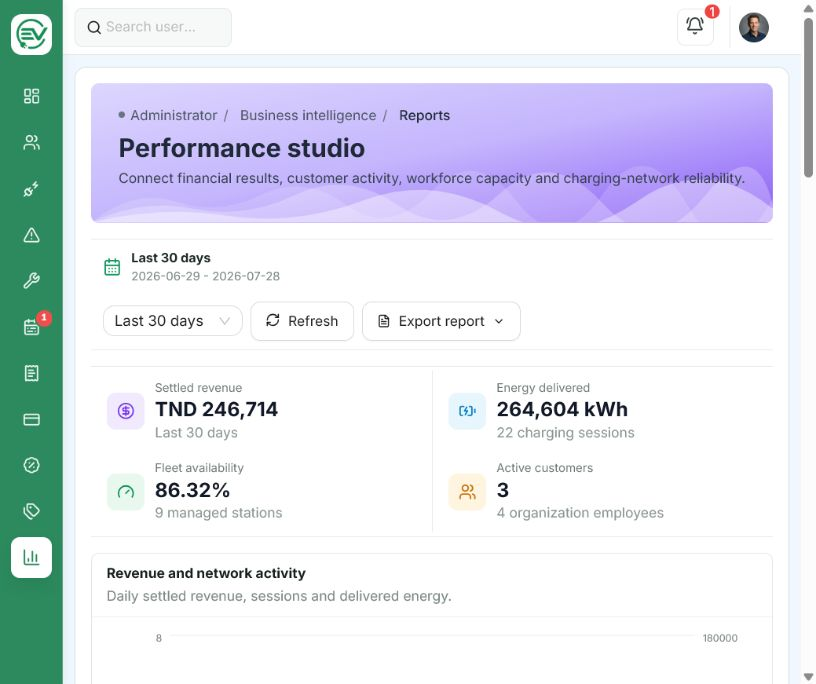
\includegraphics[width=0.94\textwidth]{assets/screenshots/administrator-reports.png}
  \caption{Analyse et rapports de l'administrateur}
  \label{fig:interfaces-admin-reports}
\end{figure}

Les exports PDF, CSV et JSON sont disponibles depuis les ressources auxquelles
ils se rapportent. Cette proximité évite de transformer la page d'analyse en
entrepôt de documents et permet de retrouver un reçu, une facture ou un rapport
d'intervention dans son workflow d'origine.

\section{Principes d'ergonomie retenus}

Les interfaces réalisées appliquent les principes suivants :

\begin{itemize}[leftmargin=7mm]
  \item conserver une navigation et une hiérarchie visuelle stables entre les
  rôles, sans exposer les fonctions non autorisées ;
  \item proposer des contrôles adaptés aux données : carte et coordonnées pour
  une position, sélecteur pour un état, calendrier pour une date et formats
  dédiés pour les exports ;
  \item afficher les états de chargement, les écrans vides et les erreurs au
  niveau du contexte concerné ;
  \item réduire les confirmations manuelles lorsque l'événement réel peut être
  observé, notamment pendant le branchement OCPP ;
  \item conserver les actions critiques explicites et demander une confirmation
  avant une suppression, un arrêt de session ou une commande distante ;
  \item adapter la densité aux écrans plus étroits sans superposer la carte, la
  barre latérale ou les panneaux de détail.
\end{itemize}

\section*{Conclusion}

Les captures montrent la continuité entre le prototype validé et l'application
fonctionnelle. L'identité visuelle demeure commune, tandis que les priorités,
les indicateurs et les actions varient réellement selon le rôle. Le chapitre
précédent établit la réalité technique des échanges OCPP, du calcul de
disponibilité et des services métier ; celui-ci montre comment ces capacités
sont rendues accessibles dans des parcours cohérents et exploitables.
